%----------------------------------------------------------------------------------
% Exemplo do uso da classe tcc.cls. Veja o arquivo .cls
% para mais detalhes e instruções.
%----------------------------------------------------------------------------------

% Seleção de idioma da monografia. Por enquanto as únicas opções
% suportadas são 'portuguese' e 'english'
% Para impressão em frente e verso, use a opção 'twoside'. Da
% mesma forma, use 'oneside' para impressão em um lado apenas.
\documentclass[portuguese,oneside]{tcc}

%----------------------------------------------------------------
% Coloque seus pacotes abaixo.
%
% Obs.: muitos pacotes de uso comum do LaTeX, como amsmath,
% geometry e url já são automaticamente incluídos pela classe
% (veja o arquivo .cls). Isso torna obrigatória a presença destes
% no sistema para o uso desta classe, mas ao mesmo tempo o uso se
% torna mais simples.  Recomendo a instalação da versão mais
% recente da distribuição TeXLive (para Windows e UNIXes):
% www.tug.org/texlive/
%
% Pacotes e opções já incluídas automaticamente:
%
% \RequirePackage[T1]{fontenc}[2005/09/27]
% \RequirePackage[utf8x]{inputenc}[2008/03/30]
% \RequirePackage[english,brazil]{babel}[2008/07/06]
% \RequirePackage[a4paper]{geometry}[2010/09/12]
% \RequirePackage{textcomp}[2005/09/27]
% \RequirePackage{lmodern}[2009/10/30]
% \RequirePackage{indentfirst}[1995/11/23]
% \RequirePackage{setspace}[2000/12/01]
% \RequirePackage{textcase}[2004/10/07]
% \RequirePackage{float}[2001/11/08]
% \RequirePackage{amsmath}[2000/07/18]
% \RequirePackage{amssymb}[2009/06/22]
% \RequirePackage{amsfonts}[2009/06/22]
% \RequirePackage{url}
% \RequirePackage[table]{xcolor}[2007/01/21]
%----------------------------------------------------------------
% Para inserção de figuras.
\usepackage{graphicx}
% Utilize a opção 'pdftex' se você estiver usando o pdflatex (que
% permite figuras em formatos como .jpg ou .png)
%\usepackage[pdftex]{graphicx}

% Para tabelas com elementos ocupando mais de uma linha
\usepackage{multirow}
% Para frações na mesma linha (ex. ⅓).
\usepackage{nicefrac}
% Para inserir figuras lado a lado.
\usepackage{subfigure}
% Para formatar algoritmos.
% A opção [algo2e] é necessária para evitar conflitos
% com as definições da classe.
%\usepackage[algo2e]{algorithm2e}
\usepackage{algorithmic}
% Um float do tipo algoritmo. No momento
% este pacote é incompatível com a classe.
%\usepackage{algorithm}

\newcommand{\ie}{{\it i.e.}}
\newcommand{\eg}{{\it e.g.}}
\newcommand{\etc}{{\it etc.}}
\newcommand{\etal}{{\it et al.}}

\newcommand{\R}{\mathbb{R}}

\usepackage{todonotes}
\newcommand\frm[2][noinline]{\todo[author=FRM,color=red!75,size=tiny,#1]{{#2}}}

%----------------------------------------------------------------
% Parâmetros customizados sob demanda
%----------------------------------------------------------------
\emergencystretch=1em   % Para evitar erro do tipo "overfull hbox"


%----------------------------------------------------------------
% Autor (OBRIGATÓRIO)
%----------------------------------------------------------------
\author{Felipe da Silva Angnes}

%----------------------------------------------------------------
% Título (OBRIGATÓRIO). Devem ser passados DOIS parâmetros,
% o título em português E o inglês, não importando o idioma
% escolhido. Os títulos são utilizados para a montagem da capa,
% resumo e abstract mais tarde.
%----------------------------------------------------------------
\title{Seu título em português aqui}
      {Your title in english here}

%----------------------------------------------------------------
% Opções para o tipo de trabalho (OBRIGATÓRIO)
%----------------------------------------------------------------
\tipotrabalho{\ptci}         % Proposta de Trabalho de Conclusão
%\tipotrabalho{\tci}         % Trabalho de Conclusão I
%\tipotrabalho{\tcii}        % Trabalho de Conclusão II

%----------------------------------------------------------------
% Seleção do curso ("este trabalho é um requisito parcial para
% obtenção do grau de (mestre ou doutor) em Ciência da Computação").
%----------------------------------------------------------------
%\curso{\cc} % Ciência da Computação
%\curso{\si} % Sistemas de Informação
%\curso{\es} % Engenharia de Software
\curso{\ec} %Engenharia de Computação

%----------------------------------------------------------------
% Orientador (e Co-orientador, caso haja um). É OBRIGATÓRIO
% informar pelo menos o orientador.
%----------------------------------------------------------------
\orientador{Felipe Meneguzzi}
%\coorientador{Ciclano de Farias}

%----------------------------------------------------------------
% A capa é inserida automaticamente. Por isso não é necessário
% chamar \maketitle
%----------------------------------------------------------------
\begin{document}

%----------------------------------------------------------------
% Depois da capa vem a dedicatória e a epígrafe.
%----------------------------------------------------------------
%\dedicatoria{Dedico este trabalho a meus pais.}

%\epigrafe{The art of simplicity is a puzzle of complexity.}
%         {Douglas Horton}

%----------------------------------------------------------------
% Também dá para fazer as duas na mesma página:
%----------------------------------------------------------------
%\dedigrafe{Dedico este trabalho a meus pais.}
%          {The art of simplicity is a puzzle of complexity.}
%          {Douglas Horton}

%----------------------------------------------------------------
% A seguir, a página de agradecimentos (OPCIONAL):
%----------------------------------------------------------------
% \begin{agradecimentos}
% À lorem ipsum, dolor sit amet consetetur sadipscing elitr sed diam
% nonumy eirmod tempor. invidunt ut labore et dolore magna aliquyam

% À erad sed, diam voluptua at vero, eos et accusam et justo duo
% dolores et ea rebum stet clita.

% À kasd gubergren, no sea. takimata sanctus est lorem ipsum dolor sit
% amet lorem ipsum dolor sit amet. consetetur sadipscing elitr sed

% À diam nonumy, eirmod tempor, invidunt ut labore et dolore magna
% aliquyam erat sed diam voluptua at.
% \end{agradecimentos}

%----------------------------------------------------------------
% Resumo, com as palavras-chave passadas por parâmetro
% (OBRIGATÓRIO, ao menos para teses e dissertações)
%----------------------------------------------------------------
\begin{resumo}{lorem, ipsum, dolor, sit, amet}
Seu resumo em português aqui. lorem ipsum dolor sit amet
consetetur sadipscing elitr sed diam nonumy eirmod tempor invidunt
ut labore et dolore magna aliquyam erat sed diam voluptua at vero
eos et accusam et justo duo dolores et ea rebum stet clita.  kasd
gubergren no sea takimata sanctus est lorem ipsum dolor sit amet
lorem ipsum dolor sit amet consetetur sadipscing elitr sed diam
nonumy eirmod tempor invidunt ut labore et dolore magna aliquyam
erat sed diam voluptua at.
\end{resumo}

%----------------------------------------------------------------
% Abstract, com as palavras-chave passadas por parâmetro
% (OBRIGATÓRIO, ao menos para teses e dissertações)
%----------------------------------------------------------------
\begin{abstract}{lorem, ipsum, dolor, sit, amet}
Your abstract in English here. lorem ipsum dolor sit amet
consetetur sadipscing elitr sed diam nonumy eirmod tempor invidunt
ut labore et dolore magna aliquyam erat sed diam voluptua at vero
eos et accusam et justo duo dolores et ea rebum stet clita kasd
gubergren no sea takimata sanctus est lorem ipsum dolor sit amet
lorem ipsum dolor sit amet consetetur sadipscing elitr sed diam
nonumy eirmod tempor invidunt ut labore et dolore magna aliquyam
erat sed diam voluptua at
\end{abstract}

%----------------------------------------------------------------
% Listas e sumário, nessa ordem. Somente o sumário é obrigatório,
% portanto, comente as outras listas, caso sejam desnecessárias.
%----------------------------------------------------------------
\listoffigures       % Lista de figuras      (OPCIONAL)

%\listoftables        % Lista de tabelas      (OPCIONAL)
%\listofalgorithms    % Lista de algoritmos   (OPCIONAL)
\listofacronyms      % Lista de siglas       (OPCIONAL)
%\listofabbreviations % Lista de abreviaturas (OPCIONAL)
%\listofsymbols       % Lista de símbolos     (OPCIONAL)
\tableofcontents     % Sumário               (OBRIGATÓRIO)

%----------------------------------------------------------------
% Aqui começa o desenvolvimento do trabalho. Para uma melhor
% organização do documento, separe-o em arquivos,
% um para cada capítulo. Para isso, utilize o comando \include,
% como mostrado abaixo.
%----------------------------------------------------------------
%----------------------------------------------------------------------------------
% Exemplo do uso da classe tcc.cls. Veja o arquivo .cls
% para mais detalhes e instruções.
%----------------------------------------------------------------------------------

% PARA PREENCHIMENTO DO REVISOR:
% CHECKLIST
% [ ] Introduction: check the introduction 
    % [ ] Avoid jargon: Do you avoid jargon that is only explain in the rest of the text?
    % [ ] Clarity: Can anyone from computer science read the introduction and understand what's the objective?
    % [ ] Does it clearly describe the problem?
    % [ ] Does the introduction clearly state the contributions?

\sigla{COLREGS}{Collision Regulations at Sea}
\sigla{LSA}{Laboratório de Sistemas Autônomos}
\sigla{USV}{Unmanned Surface Vehicle}
\sigla{VO}{Velocity Obstacles}

\chapter{Introdução}\label{chap1:intro}
    É significativo o número de importantes atividades aquáticas realizadas por seres humanos utilizando embarcações~\cite{LIU201671}. Porém, tais tarefas podem ser longas e entediantes, dificultando a constância de foco que deve ser mantida durante a execução~\cite{JURAK2020}. A distração pode levar a sérias consequências em um cenário onde há diversas embarcações na mesma área. Investigações mostram que o fator humano~\cite{HUANG2020451}, junto com o descumprimento de regras marítimas de evasão de colisão (COLREGS - do inglês \textit{"COLlision REGulations at Sea"})~\cite{JURAK2020}, são as principais causas de acidentes envolvendo embarcações.
    Visando eliminar o fator humano e possibilitando a realização de tarefas longas, perigosas e com maior precisão, estudos sobre veículos de superfície não tripulados (USV - do inglês \textit{"Unmanned Surface Vehicle"}) vêm ganhando atenção~\cite{LIU201671}.
    
    USV é um veículo que se move de forma autônoma através de um sistema embarcado ou distribuído~\cite{SONG2018351}. Com o desenvolvimento de USVs e sua atuação em meios comuns a outras embarcações (TS - do inglês \textit{"Target Ship"}), tripuladas ou não tripuladas, é inevitavel que situações de colisão aconteçam. O principal desafio, atualmente, no desenvolvimento de um USV consiste em torná-lo capaz de evitar colisões. Contudo, apenas evitar colisão não é suficiente, é preciso que o USV se movimente de acordo com as mesmas regras aplicadas aos seres humanos, ou seja, de acordo com as COLREGS~\cite{JURAK2020}. É importante que essa diretiva seja considerada no desenvolvimento de USVs, visto que em um cenário de colisão eminente entre um USV e um TS, a outra embarcação deve ser capaz de identificar a movimentação do USV como uma evasão da colisão~\cite{KUWATA2014110}.
    
    Apesar de importantes, as COLREGS são normas destinadas à compreensão de seres humanos e deixam margens para interpretação, fazendo com que uma COLREGS possa ser aplicável, ou não, dependendo de cada caso~\cite{KUWATA2014110}. Consequentemente, em um cenário onde múltiplas embarcações possuem trajetos que se cruzam em algum ponto, é desejável que o sistema de um USV seja capaz de prever se em algum momento haverá risco de colisão com alguma embarcação próxima. Nesse sentido, um método muito utilizado para verificar risco de colisão é o CPA (do inglês \textit{"Closest Point of Approach"}), onde é analisada a distância entre as embarcações no momento em que elas estarão mais próximas~\cite{HUANG2019142}. Se essa distância não for considerada segura, um risco de colisão é detectado e um procedimento de evasão deverá ser iniciado.
    
    Com base nas informações apresentadas, o presente trabalho visa desenvolver uma aplicação capaz de detectar o CPA e identificar qual encontro previsto na COLREGS é aplicável. Ademais, será realizada a integração em um sistema para USV já existente, para que seja possível realizar simulações e analisar se o comportamento resultante está de acordo com o esperado. O presente documento está estruturado da seguinte forma: no capítulo \ref{chap1:intro}, além das informações já apresentadas, o trabalho proposto será aprofundado na sessão \ref{subchap1:trab_prop}, e as contribuições serão evidenciadas na sessão \ref{subchap1:contrib}. O capítulo \ref{chap2:fund_teo} contém uma revisão teórica apresentando maiores detalhes a respeito de USV na sessão \ref{subchap2:USV}, COLREGS na sessão \ref{subchap2:colregs} e prevenção de colisão na sessão \ref{subchap2:prev_col}.
    
    \section{Trabalho Proposto}\label{subchap1:trab_prop}
        Motivado pela vontade de experienciar o processo científico, este trabalho se propõe a realizar uma breve revisão da literatura sobre evasão de colisão aplicado a USV, identificando as técnicas utilizadas atualmente. Como resultado do estudo, será desenvolvida uma aplicação que seja capaz de detectar o CPA entre um USV e um TS prevendo qual regra da COLREGS será aplicável ao encontro. Por fim, para que seja possível analisar o comportamento resultante da implementação, a aplicação será integrada a um sistema para USV já existente, desenvolvido por Jurak~\cite{JURAK2020}.
        
        Jurak~\cite{JURAK2020} desenvolveu um sistema de código aberto para evasão de colisão com respeito à COLREGs para veículos não-tripulados que navegam na superfície da água. Seu trabalho foi realizado utilizando o framework de desenvolvimento ROS (do inglês \textit{"Robot Operating System"}) e utilizou o simulador USV\_sim para realizar seus testes e obter seus resultado. Com base nisso, este trabalho será desenvolvido com base nos mesmos paradigmas ROS para que haja compatibilidade com o sistema de Jurak~\cite{JURAK2020}, possibilitando a integração. Consequentemente, o mesmo simulador será utilizado para realização dos testes.
        
    \section{Contribuições}\label{subchap1:contrib}
        A primeira contribuição deste trabalho é capacitar o sistema desenvolvido por Jurak~\cite{JURAK2020} a calcular o CPA, para que possa ser utilizado nos barcos-robôs pertencentes ao Laboratório de Sistemas Autônomos da PUCRS. Além disso, a maioria dos sistemas desenvolvidos para USVs ou são resguardados por patentes, ou então possuem acesso restrito àqueles que não participaram de seu desenvolvimento.~\cite{JURAK2020} Sendo assim, este trabalho visa contribuir à comunidade de desenvolvedores mantendo o que for desenvolvido em código aberto.
        
        A segunda contribuição, em decorrência da primeira, será identificar encontros em que as COLREGS não são aplicáveis. Kuwata \etal nos mostra, através da Figura
        
        % Contribuições previamente listadas, serão melhor trabalhadas em um texto apropriado.
        
        % \begin{itemize}
        %     \item Adicionar CPA
        %     \item Com o CPA será possível identificar situações onde a COLREGS pode ser aplicável ou não
        %     \item Com a capacidade de identificar colisões com VO, há a possibilidade de aprimorar o sistema para suportar encontro com múltiplas embarcações. Só teria que ver como ficaria a sincronia entre o VO e o método ATC (presente no sistema atualmente).
        % \end{itemize}
%----------------------------------------------------------------------------------
% Exemplo do uso da classe tcc.cls. Veja o arquivo .cls
% para mais detalhes e instruções.
%----------------------------------------------------------------------------------
\chapter{Fundamentação Teórica}\label{chap2:fund_teo}
    \section{USV}\label{subchap2:USV}
        \textit{"Unmanned Surface Vehicle"}, ou veículo de superfície não tripulado, é caracterizado por realizar atividades navais de forma autônoma, ou controlado remotamente, sem a presença de tripulação.~\cite{LIU201671} Tais caracteríscticas também enquadram um USV na categoria de um robô.~\cite{JURAK2020}
        
        De acordo com Liu~\cite{LIU201671}, um USV pode ter as mais variadas aparências e funcionalidades, porém os seguintes componentes básicos devem compor um USV:
        
        \begin{enumerate}
            \item Casco e estruturas mecânicas auxiliares
            \item Sistema de Propulsão
            \item Sistema GNC (\textit{"Guidance Navigation and Control"})
            \item Sistema de Comunicação
            \item Equipamento de Coleta de Dados
            \item Estação de Solo
        \end{enumerate}
        
        Dentre os elementos listados o sistema GNC é fundamental para automatizar um USV, pois ele controlará o sistema do USV como um todo. Sua função consiste coletar informações a respeito do USV e seu entorno (\textit{"Navigation"}), determinar o melhor caminho a seguir com base nos dados coletados (\textit{"Guidance"}) e executar as ações necessárias para seguir a melhor rota encontrada (\textit{"Control"}).  ~\cite{LIU201671} ~\cite{JURAK2020}
        
        \begin{figure}
            \centering
            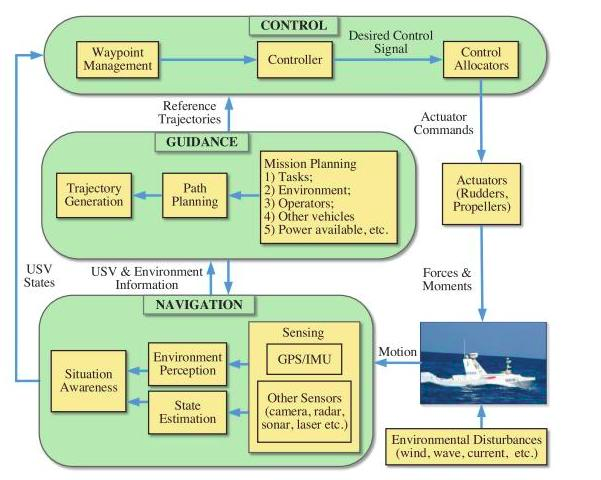
\includegraphics[width=\textwidth]{fig/gnc_system.png}
            \caption{Caption}
            \label{fig:gnc_system}
        \end{figure}
    
        A Figura ~\ref{fig:gnc_system} apresentada por Liu ~\cite{LIU201671} mostra o sistema GNC em detalhe apontando suas funções. Tais funções serão brevemente explicadas a seguir.
        
        \begin{enumerate}
            \item [1] \textit{"Navigation":} subsistema responsável pela coleta de informações a respeito do barco (posição, velocidade, etc) e seu entorno (obstáculos estáticos e obstáculos móveis). Essas informações são coletadas por meio de sensores, radares, câmeras, cartas náuticas e mapas. Os dados coletados são enviados para o subsistema \textit{"Guidance"}.~\cite{JURAK2020}
            
            \item [2] \textit{"Guidance":} subsistema reponsável por analisar os dados recebidos do subsistema \textit{"Navigation"} e encontrar o melhor trajeto possível, através de planejadores, para atingir o objetivo.~\cite{JURAK2020} Portanto, é responsabilidade do subsistema \textit{"Guidance"} executar todas as etapas necessárias para a prevenção de colisão~\cite{HUANG2020451}, que serão abordadas na sessão ~\ref{subchap2:prev_col}.
            
            \item [3] \textit{"Control":} subsistema que origina os comandos necessários para seguir a rota traçada pelo subsistema \textit{"Guidance"}. Além disso, também é sua responsabilidade executar os comandos gerados diretamente nos atuadores do USV.~\cite{JURAK2020}
        \end{enumerate}
    
    \section{COLREGS}\label{subchap2:colregs}
        Buscando padronizar as ações tomadas para evitar colisões a Organização Internacional da Marinha (IMO - do inglês International Marine Organization) definiu uma série de regulamentações para colisão no mar (COLREGS - do inglês COLlision REGulations at Sea).~\cite{JURAK2020}
        
        Para que o uso de USV não apresente perigo para outras embarcações triupuladas, é necessário que ele não realize ações inesperadas pelos humanos do barco que se aproxima. Sendo assim, o USV deverá realizar suas ações de acordo com a COLREGS de forma que seja perceptível para o humano que estiver no outro barco.~\cite{KUWATA2014110}
        
        Jurak~\cite{JURAK2020} em seu sistema considerou os seguintes encontros: 
        
        \begin{enumerate}
            \item [1] \textit{"head-on":}
            \item [2] \textit{"crossing from left"}
            \item [3] \textit{"crossing from right"}
            \item [4] \textit{"overtaking"}
        \end{enumerate}
        
        
        
    
    \section{Prevenção de Colisão}\label{subchap2:prev_col}
        Uma tarefa primordial quando se trata de navegação é evitar que a embarcação colida com algum obstáculo. Porém, é alto o número de acidentes com embarcações envolvendo colisões. Além disso, diversas investigações apontam que a principal causa desses acidentes é o fator humano.~\cite{HUANG2020451}
        
        Frente ao alto número de ocorrencias dessa natureza, pesquisadores vem estudando meios de evitar tais acidentes. [Huang] afirma que atualmente há duas frentes na tecnologia de prevenção de colisão: (1) assitência à tripulação e (2) eliminação de fatores humanos. Sendo esta última a perspectiva abordada neste trabalho dado que o componente físico de implementação é um USV.~\cite{HUANG2020451}
        
        Huang (2020, p.2) define prevenção de colisão como:
        \begin{directcite}
            \textit{"Prevenção de colisão é o processo em que um navio desvia de sua trajetória planejada para evitar contato físico indesejado em um certo tempo futuro"}
        \end{directcite}
        
        Com isso, [Huang] separa o processo de prevenção de colisão nas etapas de "detecção de conflito", que determina se o navio está em risco de colisão ou não, e "resolução de conflito", que define quais ações devem ser tomadas pelo navio para evitar a colisão. Em um USV, tais atividades são atribuidas ao módulo de \textit{"Guidance"} do sistema GNC.~\cite{HUANG2020451}
        
        Na Figura~\ref{fig:col_avoid_info_flow} é possível observar o fluxo de informação por entre os módulos que compõe um sistema de evasão de colisão. Em suma, o módulo \textit{"Observer"} coleta informações através de seus sensores e câmeras; \textit{"Motion Prediction"} faz uso dos dados coletados pelo módulo anterior para estimar as futuras posições do OS e do TS; \textit{"Conflict Detection"} ineterpreta as informações fornecidas pelos módulos anteriores para verificar se há o risco de colisão; havendo risco de colisão, o módulo \textit{"Conflict Resolution"} é acionado para determinar as ações necessárias para evadir da situação de risco; o módulo \textit{"Actuator"} executa as ações definidas pelos módulos anteriores.~\cite{HUANG2020451}
        
        \begin{figure}
            \centering
            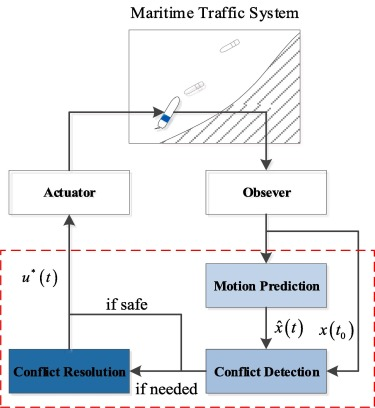
\includegraphics{fig/information_flow.png}
            \caption{Fluxo de informação ~\cite{HUANG2020451}}
            \label{fig:col_avoid_info_flow}
        \end{figure}
        
        Os módulos envoltos ao pontilhado vermelho na Figura~\ref{fig:col_avoid_info_flow} formam o sistema de evasão de colisão. 

%----------------------------------------------------------------
% Aqui vai a bibliografia. Existem 3 estilos de citação: use
% 'tcc-alpha' para citações do tipo [Abc+] ou [XYZ] (em ordem
% alfabética na bibliografia), 'tcc-num' para citações
% numéricas do tipo [1], [20], etc., em ordem de referência e
% 'tcc-alpha-full' para citações estilo 'alpha' mas com nomes completos.
%----------------------------------------------------------------
%\bibliographystyle{tcc-alpha}
\bibliographystyle{tcc-num}
\bibliography{tcc_proposta_bib}

%----------------------------------------------------------------
% Após \appendix, se iniciam os capítulos de Apêndice, com
% numeração alfabética.
%----------------------------------------------------------------
%\appendix
%\chapter{Meu primeiro apêndice}
%\chapter{My second appendix}

%----------------------------------------------------------------
% Aqui vão os "capítulos" de anexos. Cada anexo deve
% ser considerado um capítulo.
%----------------------------------------------------------------
%\anexos
%\chapter{Meu primeiro anexo}
%\chapter{My second attachment}

% E aqui (para a felicidade de todos) termina o documento.
\end{document}
